\documentclass[letterpaper,10pt]{article}

\usepackage{enumitem}
\usepackage{titling}
\usepackage{listings,listings-rust}
\usepackage{url}
\usepackage{soul}
\usepackage{hyperref}
\usepackage{setspace}
\usepackage{subfig}
\usepackage{sectsty}
\usepackage{pdfpages}
\usepackage{colortbl}
\usepackage{multirow}
\usepackage{multicol}
\usepackage{relsize}
\usepackage{amsmath}
\usepackage{wasysym}
\usepackage{fancyvrb}
\usepackage[yyyymmdd]{datetime}
\usepackage{amsmath,amssymb,amsthm,graphicx,xspace}
\usepackage[titlenotnumbered,noend,noline]{algorithm2e}
\usepackage[compact]{titlesec}
\usepackage{XCharter}
\usepackage[T1]{fontenc}
\usepackage[scaled]{beramono}
\usepackage[normalem]{ulem}
\usepackage{booktabs}
\usepackage{tikz}
\usetikzlibrary{arrows.meta,automata,shapes,trees,matrix,chains,scopes,positioning,calc,decorations.pathreplacing}
\tikzstyle{block} = [rectangle, draw, fill=blue!20, 
    text width=2.5em, text centered, rounded corners, minimum height=2em]
\tikzstyle{bw} = [rectangle, draw, fill=blue!20, 
    text width=4em, text centered, rounded corners, minimum height=2em]

\definecolor{namerow}{cmyk}{.40,.40,.40,.40}
\definecolor{namecol}{cmyk}{.40,.40,.40,.40}
\renewcommand{\dateseparator}{-}

\let\LaTeXtitle\title
\renewcommand{\title}[1]{\LaTeXtitle{\textsf{#1}}}

\lstset{basicstyle=\footnotesize\ttfamily,breaklines=true}

\newcommand{\CPP}{C\nolinebreak\hspace{-.05em}\raisebox{.4ex}{\tiny\bf +}\nolinebreak\hspace{-.10em}\raisebox{.4ex}{\tiny\bf +}}
\def\CPP{{C\nolinebreak[4]\hspace{-.05em}\raisebox{.4ex}{\tiny\bf ++}}}

\newcommand{\handout}[5]{
  \noindent
  \begin{center}
  \framebox{
    \vbox{
      \hbox to 5.78in { {\bf ECE459: Programming for Performance } \hfill #2 }
      \vspace{4mm}
      \hbox to 5.78in { {\Large \hfill #4  \hfill} }
      \vspace{2mm}
      \hbox to 5.78in { {\em #3 \hfill \today} }
    }
  }
  \end{center}
  \vspace*{4mm}
}

\newcommand{\lecture}[3]{\handout{#1}{#2}{#3}{Lecture#1}}
\newcommand{\tuple}[1]{\ensuremath{\left\langle #1 \right\rangle}\xspace}

\addtolength{\oddsidemargin}{-1.000in}
\addtolength{\evensidemargin}{-0.500in}
\addtolength{\textwidth}{2.0in}
\addtolength{\topmargin}{-1.000in}
\addtolength{\textheight}{1.75in}
\addtolength{\parskip}{\baselineskip}
\setlength{\parindent}{0in}
\renewcommand{\baselinestretch}{1.5}
\newcommand{\term}{Winter 2020}

\singlespace


\begin{document}

\lecture{21 --- GPU Programming (CUDA) }{\term}{Patrick Lam \& Jeff Zarnett}

\section*{GPUs: Heterogeneous Programming}

The next part will be about programming for heterogeneous
architectures. In particular, we'll talk about GPU programming, as
seen in CUDA. The general idea is to
leverage vector programming; vendors use the term SIMT (Single
Instruction Multiple Thread) to describe this kind of
programming. We've talked about the existence of SIMD instructions
previously, but now we'll talk about leveraging SIMT more
consciously. We are again in the domain of embarrassingly parallel
problems.

\paragraph{Cell, CUDA, and OpenCL.} 
Other examples of heterogeneous programming include
programming for the PlayStation 3 Cell~\cite{cellprimer} architecture and CUDA. (Note that the PS4 returns to a regular CPU/GPU configuration; however, it uses AMD hardware which combines the CPU and GPU on one chip.) The Cell includes a PowerPC core as well as
8 SIMD coprocessors:

\begin{center}
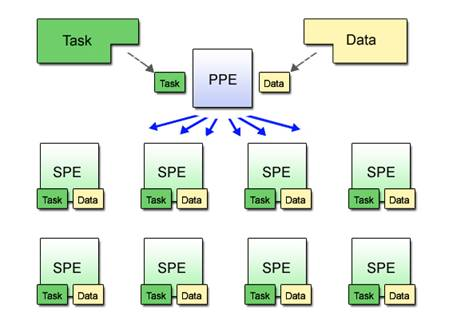
\includegraphics[width=.4\textwidth]{images/cell.jpg}
\end{center}
\hfill (from the Linux Cell documentation)

CUDA (Compute Unified Device Architecture) is NVIDIA's architecture
for processing on GPUs. ``C for CUDA'' predates OpenCL; NVIDIA still
makes CUDA tools available, and they may be faster than OpenCL on NVIDIA
hardware. On recent devices, you can use (most) \CPP~features in CUDA code,
which you can't do in OpenCL code. We used to teach OpenCL, but it seems
to be the case that CUDA has found widespread acceptance out in industry.
Hence, we use CUDA in the course. If you really need cross-platform or 
you have AMD hardware, then you want OpenCL. The principles are similar 
enough that you can take what you learned in one toolchain and apply it 
to the other.

\paragraph{Programming Model.} The programming
model for all of these architectures is similar: you write the code for
the massively parallel computation (kernel) separately from the main
code. Then at run-time, set up the data (input), transfer the data to the GPU, wait while the GPU executes the kernel, then transfer the results back. 

It makes sense to hand it over to the GPU because there are a lot of cores, although they run at a slower speed when compared to the CPU. Looking at the hardware in the ECE servers as of Fall 2020, ecetesla2 has a 4 core 3.6 GHz CPU. It also has 1920 CUDA cores that run at about 1.8 GHz. So, half the speed, but 480 times the workers. Sounds good... if the workload is suitable.

At run-time, there is significant set-up cost for interacting with the GPU and then the data transfers (input to the GPU and collecting the results) mean there is a significant overhead cost for using the GPU. But the GPU can do lots of work in parallel once it gets going. This is a lot like deciding whether to drive or fly. 

If the distance is short, say, 200 km (the distance between Ottawa and Montreal) then flying makes no sense: you have to get to the airport, be there at least an hour or two early to make your way through security checkpoints, then fly, then get from the destination airport to your final destination. Sure, the flying part is fast, but the overhead makes your total average speed not worth it.

On the other hand, if you're going a longer distance, like 4000 km (roughly the distance between Waterloo and San Francisco), then driving is way slower! Sure, the overhead of going the airport remains, but once you're in the air you're moving at 800 km/h or so and in 5.5 hours you are there. Compare that to 40 hours of driving.

CUDA includes both task parallelism and data parallelism, as we've
discussed earlier in this course. \emph{Data parallelism} is the central
feature. You are evaluating a function, or \emph{kernel},
at a set of points. Each point represents a data element, such as one of the
bodies in the n-body simulation. But you could also perform some 
transformation on each pixel of an image or each frame of a video. If you 
imagine a 2-dimensional problem, each little circle in the diagram below is
a work-item:

\begin{center}

\begin{tikzpicture}
\foreach \x in {0,0.25,...,2}
  \foreach \y in {0,0.25,...,2}
    \draw (\x, \y) circle (0.25mm);
\end{tikzpicture}
\end{center}

Another name for the set of points is the \emph{index space}. 
Each of the points corresponds to a \emph{work-item}.

CUDA also supports \emph{task parallelism}: it can run different
kernels in parallel. Such kernels may have a one-point index space. This is
doing a large number of different things in parallel. We're not really going
to focus on that and will instead stick to the part about data parallelism.

\paragraph{More on work-items.} The work-item is the fundamental
unit of work. These work-items live on an $n$-dimensional
grid (ND-Range); we've seen a 2-dimensional grid above. You may choose
to divide the ND-Range into smaller work-groups, or the system can
divide the range for you. CUDA spawns a thread for each work item,
with a unique thread ID; they are grouped into blocks. Blocks can share 
memory locally, but each block has to be able to execute independently.
That is, the system can schedule the blocks to run in any order and possibly
in parallel (we hope so!). 

You get your choice about block size. Usually, we say let the system decide. However, for some computations it's better to specify; if you do, however, you want to make best use of the hardware and use a multiple of the size of the \textit{warp}. A warp is the NVIDIA term for a unit of execution, and there can be multiple units of execution in a given GPU.

\paragraph{Shared memory.} CUDA makes lots of different types of
memory available to you:

\begin{itemize}
\item private memory: available to a single work-item;
\item local memory (aka ``shared memory''): shared between work-items
  belonging to the same work-group; like a user-managed cache;
\item global memory: shared between all work-items as well as the host;
\item constant memory: resides on the GPU, and cached. Does not change.
\item texture memory: this is global memory too, also cached, and it provides potentially a very slight speedup over using global memory. The GPU has texture memory and caches that it uses for rendering and interpolating textures, and it's available for the GPU's general-purpose operations if your use case is a match. 
\end{itemize}

Choosing which kind of memory to use is an important design decision. A simple kernel might put everything in global memory, but that's likely to be slower than making good use of local memory. It could also be tempting to put all unchanging data in the constant memory, but its space is limited, so giant vectors won't always fit.

There is also host memory (RAM in your computer), which generally contains the application's data. We will be doing explicit transfers the  of data from host memory to the GPU memory, in both directions.

\paragraph{My very own Kernel.} Let's start looking at a kernel. This is the code that will be executed by every CUDA thread somewhat in parallel. First, let's see what the code would look like if we just wrote it in \CPP:

\begin{lstlisting}[language=C++]
void vector_add(int n, const float *a, const float *b, float *c) {
  for (int i = 0; i < n; i++) {
    c[i] = a[i] + b[i];
}
\end{lstlisting}


The same code looks like this as a kernel~\cite{cuda}:
\begin{lstlisting}[language=C++]
__global__ void VecAdd(float* A, float* B, float* C)
{
    int i = threadIdx.x;
    C[i] = A[i] + B[i];
}
\end{lstlisting}

You can write kernels in a variant of \CPP, and it looks mostly like the language we (hopefully) know, with a few additions like the \texttt{\_\_global\_\_} designation in the previous example. A large number of features of more recent versions of the language are supported, but how much will vary based on your release of the kernel compiler (\texttt{nvcc}). There's a very long list of things that are not allowed in device code. It's unlikely that we'll be doing too many things that are exotic enough to be forbidden by the compile in this course. However, if you aren't sure why something isn't working or want to know what kind of stuff is not allowed, see \url{https://docs.nvidia.com/cuda/cuda-c-programming-guide/index.html#restrictions}

(Just for completeness: the kernel itself is actually compiled into a form called PTX -- Parallel Thread eXecution -- instructions. It's possible to write those directly, but we won't; we'll just let the compiler do it. Also, using the nvcc compiler makes it so your kernel will run on whatever hardware you have.)



Remember that the kernel has none of the safety guarantees that we normally get in Rust! 

\subsection*{Writing a Kernel Well}

To start with, of course, we need to decide what sort of work belongs in the kernel to begin with. Anything that would benefit from the very large number of execution units is a good candidate, so that's typically things that are the iterations of a loop. If the loops need to be sequential, though, this is not a good match. If you need a little bit of coordination, we can achieve that, though, with barriers (as we can see in the advanced section).

Comparing the first kernel that we saw against its CPU-code equivalent, we've taken the explicit for loop and made it implicit. It's possible to have up to three-dimensional problems supported. So for the N-body problem, we could have it be a one-dimensional problem where we just use the GPU on the outer loop. Or, we could instead treat each pair of points as two dimensions in the space, making it a two-dimensional problem. 


If you want something more than a three-dimensional, you have to have some loops in your code. So that 6-level-deep nested-for-loop? You can have the outer three loops as your x, y, and z dimensions, but the rest will be in for loops. Can't avoid everything, I am afraid. The limit to three dimensions is probably because graphics cards were designed for rendering images in 3-D so it seems logical? But that's only a guess.

Of course, you can sometimes flatten the dimensions of your problem a bit. A rectangular array in C/\CPP~is really stored as a linear array and the \texttt{[x][y]} is just notational convenience so you could easily just treat it as a linear array. Or, in the case of the N-Body problem, you could consider each pair of points \textit{(i, j)} to be one point in the problem space and it's linear, potentially allowing you a bit more simplicity in your kernel at the cost of slightly more complicated host code. 

\paragraph{Branches.} OpenCL implements a SIMT architecture. The documentation warns you, however, that unlike a CPU, there's neither branch prediction nor speculative execution. This means that branches are much more costly than they would be on the CPU. 

In practice, the hardware will execute all branches that any thread in
a warp executed (which can be slow). It then keeps only the results that are valid. Consider this brief pseudocode-example:

    \begin{verbatim}
kernel contains_branch(global float *a, global float *b) {
    if (condition) {
        a[id] += 5.0;
    } else {
        b[id] += 5.0;
    }
}
\end{verbatim}

In the above example, the {\tt if} statement will cause
the warp both branches of the {\tt if}, keeping only the
result that is correct. But still, unnecessary work is done and we want to
avoid that if we can. 

Similarly, executing a loop will cause the
workgroup to wait for the maximum number of iterations of the loop in
any work-item. Frequently that isn't a problem, because the loop will be executed The compiler will try to unroll loops if they have a known number of iterations. Here, an example from the CUDA docs of a loop it can unroll:

{\scriptsize \hspace*{2em} \begin{minipage}{.5\textwidth}
    \begin{lstlisting}verbatim
__device__ void foo(int *p1, int *p2) {
  for (int i = 0; i < 12; ++i) {
    p1[i] += p2[i]*2;
  }
}
    \end{lstlisting}
\end{minipage} }

If you're setting up workgroups, though, you can arrange for all
of the work-items in a workgroup to execute the same branches. 

\subsection*{Launch?}

So far, all we have covered is the theory and then how to write a kernel. To make use of it, we'll have to look at the host code. That's our next topic. 


\bibliographystyle{alphaurl}
\bibliography{459}


\end{document}
